% interactnlmsample.tex
% v1.05 - August 2017

\documentclass[]{interact}

\usepackage{epstopdf}% To incorporate .eps illustrations using PDFLaTeX, etc.
\usepackage[caption=false]{subfig}% Support for small, `sub' figures and tables
%\usepackage[nolists,tablesfirst]{endfloat}% To `separate' figures and tables from text if required
%\usepackage[doublespacing]{setspace}% To produce a `double spaced' document if required
%\setlength\parindent{24pt}% To increase paragraph indentation when line spacing is doubled

\usepackage{algorithm,algorithmic}
\usepackage{hyperref}
\usepackage{mathtools}
\usepackage{amssymb}
\usepackage{caption}
\usepackage{threeparttable}
\usepackage{tikz}
\usepackage{multirow}
\usepackage{booktabs,tabularx}
%\usepackage{subcaption}
\DeclareMathOperator{\argmaxH}{argmax} 
\DeclareMathOperator*{\argmin}{argmin}
\renewcommand{\algorithmicrequire}{\textbf{Input:}}
\renewcommand{\algorithmicensure}{\textbf{Output:}}
\newcommand\abs[1]{\left|#1\right|}

\usepackage[numbers,sort&compress]{natbib}% Citation support using natbib.sty
\bibpunct[, ]{[}{]}{,}{n}{,}{,}% Citation support using natbib.sty
\renewcommand\bibfont{\fontsize{10}{12}\selectfont}% Bibliography support using natbib.sty
\makeatletter% @ becomes a letter
\def\NAT@def@citea{\def\@citea{\NAT@separator}}% Suppress spaces between citations using natbib.sty
\makeatother% @ becomes a symbol again

\theoremstyle{plain}% Theorem-like structures provided by amsthm.sty
\newtheorem{theorem}{Theorem}[section]
\newtheorem{lemma}[theorem]{Lemma}
\newtheorem{corollary}[theorem]{Corollary}
\newtheorem{proposition}[theorem]{Proposition}

\theoremstyle{definition}
\newtheorem{definition}[theorem]{Definition}
\newtheorem{example}[theorem]{Example}

\theoremstyle{remark}
\newtheorem{remark}{Remark}
\newtheorem{notation}{Notation}
\bibliographystyle{plain}


\begin{document}

\articletype{Journal of Nuclear Science and Technology}% Specify the article type or omit as appropriate

\title{Model-order reduction of non-linear time dependent neutronics via POD-Galerkin projection and DEIM}
\author{
\name{Rabab Elzohery\thanks{CONTACT A.~N. Author. Email: rababelzohery@ksu.edu} and Jeremy Roberts}
\affil{Department of Mechanical and Nuclear Engineering,
	Kansas State University \\
	3002 Rathbone Hall, Manhattan, KS 66506, US \\ rababelzohery@ksu.edu, jaroberts@ksu.edu}
}

\maketitle
\begin{abstract}
Presented here is an application of model-order reduction to non-linear neutronic transients.
% where reduced-order models (ROMs) are generally sought to provide a rapid, yet accurate, approximation of a particular simulation response.
The effort described extends previous work\cite{elzohery2021modeling} aimed to develop and assess a ROM framework that can be used for different purposes, such as design optimization and propagating input parameter uncertainties like nuclear data.
Here, the target applications here is non-linear.
The ROM was built with the use of the POD-Galerkin projection method and the matrix version of the Discrete Empirical Interpolation Method (MDEIM) for improved efficiency.
The MDEIM is used to approximate the projection of the problem operator that otherwise must be computed at each non-linear iteration within each time step, which increases the ROM cost.
By using the MDEIM, an offline-online ROM decomposition was obtained, which is favored from a computational perspective since the expensive projection operation can take place only once in the offline stage.
The online stage, which involves solving a linear system  at each time step, depends only on the reduced dimension and is therefore cheap, making it possible to increase the solution time resolution, and accordingly accuracy, without introducing significant cost.
By applying the method to the LRA benchmark, speed ups from 6 to 40 were achieved depending on the full-order model (FOM) spatial fidelity.
The maximum relative error in the assemblies power was in the order of $1\times10^{-5}$\%.
Moreover, the ROM was parameterized by POD-greedy sampling, and a case study was performed where the kinetic data, i.e, the precursor decay constants and delayed-neutron fraction were assumed to be the model parameters of interest.
For the parameterized ROM, the maximum relative error in the assembly power was $1\times 10^{-3}$\%, which implies that the developed ROM can be reliably used to accelerate parametric and uncertainty quantification studies involving non-linear problems.
The computational gain from the MDEIM-ROM was compared with that of a direct projection ROM and showed that employing the MDEIM is computationally advantageous, and the advantage grows with dimension of the problem.
The method was implemented in the open-source deterministic transport code Detran\cite{roberts2014advanced} where only access to the system operator was needed to construct the ROM, and; hence, the method is trivially invasive and could easily be implemented in many modern deterministic diffusion codes.


\end{abstract}

\begin{keywords}
Galerkin projection; POD; Non-linear reduced-order models; Neutronic Transient; Discrete Empirical Interpolation Method
\end{keywords}


\section{Introduction}
Modeling and simulation of reactor physics is crucial to understanding nuclear reactors' behavior under different conditions and scenarios and hence ensure reliable designs and well-established safety limits.
The mathematical models governing reactor physics are described by a set of equations that are challenging to solve analytically due to the geometric complexity of nuclear reactors except for simplified cases.
Alternatively, these systems are solved by employing numerical discretization that relies on discretizing the system along each independent variable and the solution is provided only on these discrete points.
To improve the method accuracy, the system needs to be solved over a very fine mesh.
Although this results in a more reliable solution, it leads to a growing space dimension and accordingly large computational cost.
This problem of the computational cost becomes inevitably prohibitive with applications that require repetitive execution of the simulation such as uncertainty quantification, and design optimization.
In such studies, the high-fidelity model has to be solved at multiple parameter points which could be very large.
Hence, surrogate models that are cheap, yet accurate, are sought to provide a rapid and reliable approximation of the solution of these systems.
The premise is that this lower-order model will capture the essential features of the system and preserve the input-output mapping as much as possible.

In the application of our interest here, neutronic transients, the mathematical models are based on the diffusion approximation and the Boltzmann transport equation.
For realistic modeling, these neutron transport models need to be coupled with different physics models to account for their feedback.
For example, thermal-hydraulics feedback plays an essential role in reactor operation.
Changes in the fuel temperature alter the cross sections due to Doppler broadening \cite{stacey2018nuclear}, which in turn impacts the neutron population and hence the fission rate and the rate of heat generation.
Multi-physics modeling accounts for these different feedback mechanisms; however, it poses a challenge in terms of the computational cost,
since it entails solving coupled systems for different fields such as neutron flux, temperature, and flow rate.
Moreover, the neutron transport (or diffusion) equation is no longer a linear one due to the indirect dependence of the cross section on the neutron flux.
Two approaches are used to solve such systems.
The most commonly used one is a serial coupling of two or more separate codes in such a way that the output of one at a given time step, such as the flux distribution, is used as an input to the other, e.g., the temperature (which can be used then to update the cross section and so on).
This procedure is commonly referred to as operator splitting or explicit coupling.
One drawback of operator splitting is that time integration requires small steps to avoid stability issues, thus leading to high computational time. 
Alternatively, tight coupling in time between the physics can be maintained by using an implicit scheme that solves a non-linear iteration in each time step, also increasing the computational time.
A modern algorithm such as Jacobian free Newton-Krylov (JFNK) \cite{gaston2009parallel} can be used to perform this implicit coupling.
Another popular approach is to use fixed-point iteration, with an implicit time scheme to iterate between difference physics within a time step until convergence is satisfied, which is computationally taxing.
The aim of this work is to use a reduced-order model to overcome the high computational expense of these non-linear models.
In particular, the ROM was developed using the POD-Galerkin projection.
The method belongs to the projection-based family and can be described as a physics-driven method since it requires knowledge of the original governing equation as will be shown in Sec.\ref{sec:POD}.
In a previous work \cite{elzohery2021modeling}, we applied the method to the time-dependent diffusion equation where there was no coupling with other models and hence the application was linear.
In this study, the developed ROM was extended to treat the non-linearity induced by multi-physics modeling.
To improve the computational efficiency of the developed ROM, a hyper-reduction technique known as the Discrete Empirical Interpolation Method (DEIM) was used in conjunction with the POD-Galerkin projection.
The primary purpose of using the DEIM is to obtain an offline-online decomposition of the ROM to avoid repetitive projection of the problem operator at each iteration within the time step.
The offline stage occurs only once and comprises the expensive step of the ROM.
On the other hand, the online stage involves solving a reduced number of equations at each time step with a computational cost independent of the FOM dimension and hence cheaper.
The LRA benchmark was used as a demonstrative application where the diffusion equation is coupled with a simplified thermal feedback model.

%The following discussion include a general overview of the methods and algorithms, then the specific application was described after which its results are presented. 

%--------------------------------------------------------------------------------------------------%
\section{Methods Overview}

In this section, the methods used throughout the study are described, including the POD-Galerkin projection used to build the ROM, DEIM used to improve the computational efficiency of the ROM, and greedy POD sampling used to parameterize the ROM.

%--------------------------------------------------------------------------------------------------%

\subsection{POD-Galerkin Projection}\label{class}

Consider the following dynamic system that results from the discretization a partial differential equation using, e.g, the finite-difference method:
\begin{equation}
	\frac{d\mathbf{y}(t)}{dt} = \mathbf{A}\mathbf{y}(t) + \mathbf{f}(\mathbf{y}(t)),  \quad\quad \mathbf{y(0) = \mathbf{y_0}} \, ,
	\label{eq:FOM}
\end{equation}
where $\mathbf{y} \in \mathbb{R}^{n}$ is the state variable and $\mathbf{A} \in \mathbb{R}^{n\times n}$ is the operator resulting from the system discretization.
In general, this method involves two main steps.
First, a subspace is obtained using proper orthogonal decomposition (POD)\cite{volkwein2011model}.
Commonly, the POD subspace is generated using the snapshots method \cite{sirovich1987turbulence} by constructing a data matrix $\mathbf{Y}$ containing the system solutions at different times of which the singular value decomposition (SVD) is computed, i.e, $\mathbf{Y} = \mathbf{U}\mathbf{\Sigma}\mathbf{V}^T$.
The POD subspace is the one spanned by the first $r$ vectors of $\mathbf{U}$, where $r \ll n$.
There is no general \textit{a priori} rule based on which the rank $r$ is chosen; however, one can set a threshold $\epsilon$  such that
\begin{equation}
	\frac{\sum_{i=0}^r S_i}{\sum_{i=0}^m S_i} \ge \epsilon \, ,
\end{equation}
where S$_i$ is the $i$th singular value and the singular values are the elements of the diagonal matrix $\mathbf{\Sigma}$.
Upon obtaining the reduced space, the state variable $\mathbf{y}$ is expanded in terms of its basis
\begin{equation}
	\mathbf{y} \approx \mathbf{U} \hat{\mathbf{y}}(t) \, ,
	\label{eq:galerkin expansion}
\end{equation}
where $\mathbf{\hat{y}(t)} \in \mathbb{R}^{r}$ is a vector of the temporal coefficients.
Second, the system is projected onto a POD subspace by multiplying the system on the left by $\mathbf{U}^T$ and making use of the orthogonality of the POD basis (i.e, $\mathbf{U}^T\mathbf{U} = \mathbf{I}$), which leads to
\begin{equation}
	\frac{d\mathbf{\hat{y}}}{dt} = \mathbf{A}_r\mathbf{\hat{y}} + \mathbf{U}^T\mathbf{f}(\mathbf{U}\mathbf{\hat{y}})\, ,  \qquad \mathbf{\hat{y}}(0) = \mathbf{U}^T\mathbf{y}_0 \, ,
	\label{eq:ROM}
\end{equation}
where $\mathbf{A}_r \in \mathbb{R}^{r\times r} = \mathbf{U}^T\mathbf{A}\mathbf{U}.$
Thus, we are left with $r$ ODE's instead of $n$ ODE's, which makes the resulting ROM cheaper to solve, and once it is solved for $\mathbf{\hat{y}}$, the full order solution can be computed by Eq.~\ref{eq:galerkin expansion}.

%--------------------------------------------------------------------------------------------------%

\subsection{Discrete Empirical Interpolation Method}

\label{sec:DEIM}
Recently, the DEIM \cite{chaturantabut2010nonlinear} was proposed to approximate the non-linearity in the context of model-order reduction and to facilitate the online/offline decomposition of ROMs.
The method is a discrete variant of the Empirical Interpolation Method (EIM) \cite{barrault2004empirical} that was originally proposed to approximate non-affine coefficient functions using a reduced-basis expansion to facilitate the online/offline decomposition in finite-element methods.
To illustrate the method, consider the model in Eq.\ref{eq:FOM} for which we seek an approximate ROM.
The non-linear term $\mathbf{f}(\textbf{y}(t))$ introduces computational complexity to the ROM since computing the projected term $\mathbf{U}^T\mathbf{f}(\textbf{y}(t))$ requires reconstructing the full-order  solution first.
The reconstruction and the projection steps have costs dependent on the dimension of the system $n$.
The goal of using the DEIM is to avoid performing these operations at each time step by splitting the ROM into two steps: an offline step in which the expensive operations dependent on $n$ are performed, and an online step in which operations depend only on the reduced dimension.
The method relies on two main ingredients: (1) a reduced space in which nonlinear function can be approximated, and (2) a set of spatial interpolation indices.
The nonlinear function $\mathbf{f}(\textbf{y}(t))$ is approximated by projecting it onto a subspace that approximates the function space
\begin{equation}
	\mathbf{f}(\textbf{y}(\tau)) = \mathbf{\Psi}\boldsymbol{\theta}(\tau)\, ,
\end{equation}
where $\mathbf{\Psi} \in \mathbb{R}^{n\times k}$ is a low-dimensional subspace with $k \ll n$, and $\boldsymbol{\theta}(\tau) \in \mathbb{R}^k$ is a vector of the corresponding coefficients.
POD is used to find the subspace $\mathbf{\Psi}$ using snapshots of the function (i.e, $[\textbf{y}(t_1), ....., \textbf{y}(t_m)]$).
In order to compute $\theta(t)$, a few spatial indices are selected iteratively using a greedy search following Algorithm \ref{alg:DEIM}.
The basic idea is to select $k$ rows of the basis matrix $\mathbf{\Psi}$.
The algorithm takes as an input the basis vectors of the subspace $\mathbf{\Psi}$.
The first index is selected where the entry of the first input basis has the largest magnitude.
Each other index $\mathcal{I}_i$ is selected where the approximation of the corresponding input basis vector $\mathbf{\Psi_i}$ in the subspace constructed by interpolating the basis $[\mathbf{\Psi}_1, ....\mathbf{\Psi}_{i-1}]$ at the previously selected indices is worst.
Once the indices are selected, the matrix $\mathbf{\Psi}_k \in \mathbb{R}^{k\times k}$ is formed such that
\begin{equation}
	\mathbf{\Psi}_k = \mathbf{P}^T\mathbf{\Psi}\, ,
\end{equation}
where $\mathbf{P} = [e_{z1}, e_{z2}, ....,e_{zk}] \in \mathbb{R}^{n\times k}$ and $e_{zi} = [0,.., 0, \underbrace{1}_{{zi}}, 0..., 0]^\text{T} \in \mathbb{R}^{n}$
is the  ${zi}$th column of the identity matrix.
The coefficients can be computed by solving
\begin{equation}
	\mathbf{P}^T\mathbf{f(\tau)}=\mathbf{\Psi}_k \boldsymbol{\theta}(\tau)\, ,
	\label{eq:DEIM coefficients}
\end{equation}
and the final approximation is given by
\begin{equation}
	\hat{\mathbf{f}}(\tau)\approx\mathbf{\Psi}( \mathbf{\Psi}_k)^{-1}\mathbf{P}^T\mathbf{f} (\tau)\, .
\end{equation}
A key point relevant to the computational efficiency of the method is that the matrix $\mathbf{P}$ does not need to be constructed explicitly since the term $\mathbf{P}^T\mathbf{f}$ extracts only the elements of $\mathbf{f}$ that correspond to the interpolation indices.
Thus, at each time step, only $k$ elements $\mathbf{f}$ need to be evaluated.
%The approximation error can be bounded as 
%\begin{equation}
%	\|\mathbf{f} - \hat{\mathbf{f}} \| \le \|(\mathbf{P}\mathbf{\Psi})^{-1} \| \epsilon \, ,
%\end{equation}
%where
%\begin{equation*}
%	\epsilon \approx \sigma_{k+1} \, .
%\end{equation*}
%Note that $\sigma_{k+1}$ is the $(k+1)th$ singular value coming from the SVD of the function snapshots matrix.
%Full derivation of the error bound is given in Ref.~\cite{chaturantabut2010nonlinear}.

Now, the projection can be performed by computing the term $\mathbf{U}^T \mathbf{\Psi}$ once in an offline stage, while in the online stage, the vector $\boldsymbol{\theta}$ is computed by solving the linear system of dimension $k$ in Eq.~\ref{eq:DEIM coefficients}.
Thus, the cost of the online computation depends on the reduced dimension $k$, not the original, larger dimension $n$.

Although the problem tackled here does not include a non-linear term, the DEIM idea is exploited to approximate time-dependent operators to avoid computing the projected operator $\mathbf{A}_r(t)$ at each time step, which requires number of FLOPS dependent on $n$.
This is known as the matrix version of the DEIM, i.e, MDEIM and it was suggested in \cite{carlberg2012efficient, benner2015survey}.
To illustrate, consider the operator $\mathbf{A}(\boldsymbol{t}) \in \mathbb{R}^{n\times n}$.
The DEIM procedures can be used to approximate the operator by a summation of few time independent matrices, each weighted by a temporal coefficient.
First, the matrix can be cast in a vector form by stacking its elements in one vector $\mathbf{a}(t) \in \mathbb{R}^{n^2}$.
This vector can be treated in the same exact way as the function $\mathbf{f}(t)$ in the previous section, i.e, $\mathbf{a}(\mu) = \mathbf{\Psi}\boldsymbol{\theta}(t)$.
Snapshots of the serialized matrix are collected at different time instances and the reduced subspace $\mathbf{\Psi}$ and the interpolation indices are computed following algorithm \ref{alg:DEIM}.
Again, the corresponding coefficients are obtained by solving Eq.~\ref{eq:DEIM coefficients}. 
Next, each vector in $\mathbf{\Psi}$ can be mapped back to an $n \times n$ matrix, i.e, $\textbf{A}_i$.
Hence, the matrix is approximated as $\mathbf{\hat{A}}(t)=\sum_{i=0}^k \theta_i(t) \mathbf{A}_i$ and the projection term is computed as
\begin{equation}
	\mathbf{U}^T\mathbf{A}\mathbf{U} = \sum_{i=0}^k \mathbf{\theta}_i(t)\mathbf{U}^T\mathbf{A}_i\mathbf{U} \, .
	\label{Eq:deim matrix projection}
\end{equation}
As pointed out in Ref.\cite{negri2015efficient}, the Weyl\textendash Mirsky theorem \cite{weyl1912asymptotische} ensures that the singular values of the approximated matrix approach that of the original as $k$ increases 
\begin{equation}
	|\sigma_i - \hat{\sigma_i}  |\ \le \|\mathbf{A} - \hat{\mathbf{A}}\|_\text{F}
\end{equation}
where $\sigma_i$ and $\hat{\sigma_i}$ denote the $i$th singular value of $\mathbf{A}$ and $\hat{\mathbf{A}}$ respectively.
%Moreover, some properties of the original matrix such as positive definiteness can be preserved \cite{carlberg2015preserving}, if necessary, by imposing some constrains to the problem in Eq.~\ref{eq:DEIM coefficients}.

In practical implementations, the method efficiency can be improved, as suggested in Ref. \cite{negri2015efficient}.
First, the matrix $\mathbf{A}$ is, generally, largely sparse, which leads to a snapshots matrix that is sparse, too.
Consequently, it is more convenient to store only the nonzero elements ($nz$) in $\mathbf{a}$, 
which should be appreciably more efficient in terms of memory and computational expense.
In addition, to obtain the expansion coefficients ($\boldsymbol{\theta}$), the term $\mathbf{P}^T\mathbf{a(t)}$ needs to be computed at each new time step.
In fact, this term only extracts the elements of $\mathbf{a(t)}$ that corresponds to the selected  interpolation indices.
In the offline stage, a mapping can be done between these interpolation indices and the corresponding row-column pairs in $\mathbf{A}$.
When the matrix is formed in the online stage, only these entries are evaluated by restricting a \textit{for loop} over these row-column pairs, leading to more reduction in the computational cost.

For the rest of this paper, we will refer to the ROM with MDEIM as the MDEIM-ROM, while we refer to the model in Sec.~\ref{sec:POD} as the direct projection ROM.


\noindent\begin{minipage}{\textwidth}
	\renewcommand\footnoterule{}
	\begin{algorithm}[H]
		\caption{DEIM}
		\label{alg:DEIM}
		\begin{algorithmic}[1]
			\REQUIRE Snapshots matrix: $\mathbf{X} = [\mathbf{f}_1, \mathbf{f}_2,  ...., \mathbf{f}_m] \in \mathbb{R}^{n\times m}$
			\ENSURE A reduced space $\mathbf{\Psi}$, set of indices $\mathcal{I}$
			\STATE $[\mathbf{\Psi}_1, \mathbf{\Psi}_2, ..., \mathbf{\Psi}_k ]$ = POD(${\mathbf{X}}, \epsilon$)\footnote{POD refers to the POD procedures in Sec.~\ref{sec:POD}}
			\STATE $\mathcal{I}_1 = \argmaxH(\abs{\mathbf{\Psi}_1})$, $\mathcal{I}$ = $\{\mathcal{I}_1\}$
			\STATE $\mathbf{\Psi} = [\mathbf{\Psi}_1]$, $\mathbf{P} =[e_{I_1}]$
			\FOR {i=2 \TO i=k }
			\STATE Solve $(\mathbf{P}^T\mathbf{\Psi})\mathbf{c} = \mathbf{P}^T\mathbf{\Psi}_i$;
			\STATE $\mathcal{I}_i = \argmaxH{\abs{\mathbf{\Psi}_i - \mathbf{\Psi}\mathbf{c}}}$
			\STATE $\mathcal{I} = \mathcal{I} \cup \mathcal{I}_i$, $\mathbf{P} = \mathbf{P} \cup e_{I_i}$, ${\Psi = \Psi \cup \Psi_i}$
			\ENDFOR
		\end{algorithmic}
	\end{algorithm}
\end{minipage}

%-----------------------------------------------------------------------------------------%

\subsection{Greedy POD}
\label{sec:POD}

A greedy sampling in the parameter space \cite{nguyen2009reduced} can be combined with POD to construct a global subspace that can be used in the framework of parametric ROMs.
The primary goal is to ensure that the parameter domain of interest (i.e, $\mathbb P$) is efficiently sampled and includes enough information such that it can be used or wide range of parameters including those of higher dimensions.
To construct this subspace, a training parameters dataset, $P_{train} \subset \mathbb P$, is prepared. 
The greedy subspace is initialized with the first $r_1$ POD basis computed from a randomly selected sample of the training data.
Using this subspace, the ROM prediction error of the state variable for the rest of the training samples is computed.
The sample at which the error is worst is selected, and the subspace is enriched by adding the first $r_1$ POD basis computed from the selected sample snapshots.
Selecting the samples with the worst errors ensures efficient sampling of the parameter space.
Intuitively, samples that are close to the previously chosen parameter points will have a smaller ROM error.
On the other hand, one expects that the ROM will fail to give an accurate prediction at samples that are far from the included points in the current subspace.
Thus, we keep adding new basis vectors until a maximum size of the subspace is reached or a user-specified error tolerance at a reference parameter point $\boldsymbol{\mu}_{\text{ref}}$ is met.
Note that each time a new basis vector is added, the subspace is orthonormalized.

Regarding the error criteria based on which a new sample is selected, there are two approaches. 
Ideally, the true error can be used leading to ``strong POD-greedy'' \cite{benner2017model}.
Alternatively, an error indicator can be used to alleviate the computational burden associated with evaluating the full-order-model. 
Here, we used the strong-POD greedy approach. 
The algorithm steps are shown in Algorithm \ref{alg:greedy pod}. 
The term $\Delta(\textbf{U},\boldsymbol{\mu}_\text{ref})$  is the error measure using the current reduced subspace at $\boldsymbol{\mu}_\text{ref}$, and $r$ is the maximum size of the greedy basis.

\begin{algorithm}[H]
	
	\begin{algorithmic}
		
		\REQUIRE $\epsilon_{tol}, r, r_1, P_{train} \subset \mathbb P$ 
		
		\ENSURE A reduced space $\textbf{U}$
		
		\STATE Set n=0; randomly choose $\boldsymbol{\mu}\in P_{train}$
		\STATE Evaluate the FOM at $\boldsymbol{\mu}$, $\textbf Y(\boldsymbol{\mu})$:= $\{\textbf{y}^1, \textbf{y}^2, ..... \textbf{y}^k\}$
		\STATE $\mathbf{U} := \{\zeta_1, \zeta_2, ......,\zeta_{r1}\} := \text{POD}(\textbf{Y}(\boldsymbol{\mu}))$
		\WHILE {$\epsilon:= \Delta(\textbf{U}, \boldsymbol{\mu}_\text{ref}) > \epsilon_{tol}$ or $n < r$}
		
		\STATE $\boldsymbol{\mu} := \argmaxH_{\boldsymbol{\mu}_\in P_{train}} \Delta(\textbf{U}, \boldsymbol{\mu)}$
		
		\STATE Evaluate the FOM at $\boldsymbol{\mu}$, $\textbf Y(\boldsymbol{\mu})$:= $\{\textbf{y}^1, \textbf{y}^2, ..... \textbf{y}^k\}$ 
		
		\STATE Compute the POD modes of the FOM snapshots, $\{\zeta_1, \zeta_2, ......,\zeta_{r1}\} := \text{POD}(\textbf{Y}(\boldsymbol{\mu}), r_1)$
		
%		\STATE Compute the SVD of $\textbf Y(\mu)$ and keep the first $r_1$ POD modes:$\{\zeta_1, \zeta_2, ......,\zeta_{r1}\}= \text{POD}(\textbf{y}^1, \textbf{y}^2, ..... \textbf{y}^k\}, r_1) $
%%		
%		\STATE $Z = \{Z, \{\zeta_1, \zeta_2, ....,\zeta_{r1}\}\}$ \text{and set} $n = n+r_1$
%		
		\STATE update the reduced space, $\textbf{U} := \textbf{U} \cup \{\zeta_1, \zeta_2, ..,\zeta_{r1}\} $ and orthonormalize
		
		\STATE $n:=n+r_1$
		
		\STATE $ \textbf{compute} ~\epsilon = \Delta(\textbf{U}, \mu_0)$
		
		\ENDWHILE
		
	\end{algorithmic}
	
	\caption{POD-greedy sampling procedures}
	
	\label{alg:greedy pod}
	
\end{algorithm}

%-----------------------------------------------------------------------------------------------------%
\section{Application}

\subsection{The time-dependent diffusion equation}
\label{sec:fom}
In this work, the time dependent diffusion equation was used as the mathematical model of neutronic transients in nuclear reactors, i.e FOM, and for which an approximate ROM is sought.
The multi-group version of the equation is represented as
\begin{equation}
	\begin{split}
	\frac{1}{v_g} \frac{\partial\phi_g}{\partial t} &= 
	\nabla. D_g\nabla\phi_g - \Sigma_{tg}\phi_g + \sum_{g^\prime=1}^{G}{\Sigma_{sg^\prime g}}\phi_{g^\prime} \\
	&+ \chi_g(1-\beta)\sum_{g^\prime = 1}^{G}\nu\Sigma_{fg^\prime}\phi_{g^\prime}  
	+ \chi_g\sum_{i=1}^{P} \lambda_i C_i \, ,
	\end{split}
	\label{time_diff}
\end{equation}
where 
\begin{equation*}
	\frac{\partial C_i}{\partial t} = -\lambda_i C_i + \beta_i \sum_{g^\prime=1}^{G} \nu\Sigma_{fg^\prime} \phi_{g^\prime} \, ,
\end{equation*}
and $\phi_g$, $D_g$, $\Sigma_{ag}$, $\nu\Sigma_{fg}$ and $v_g$ are the neutron flux, diffusion coefficient, the absorption cross section, the production cross section and the average neutron velocity in group g, respectively. $\Sigma_{sg^\prime g}$ is the scattering cross section from group $g^\prime$ to group $g$ 
and $\chi_g$ is the probability that a fission neutron will be born in group $g$.
$C_i$ is the $i$th precursor concentration, $\beta_i$ is the fraction of delayed neutrons in group $i$, $\lambda_i$ is the $i$th group decay constant.
%The system can be represented compactly in a matrix form as 
%\begin{equation}
%\frac{\partial{y}(r, t)}{\partial{t}} = \mathcal{A}{y}(r, t) \, ,
%\end{equation}
%where the stacked unknowns are
%\begin{equation*}
%	{y} = 
%	\begin{pmatrix}
%	\phi_1(r, t) \\
%	\vdots \\
%	\phi_G(r, t)  \\
%	{C}_1(r, t) \\
%	\vdots \\
%	{C}_I(r, t) \\
%	\end{pmatrix} \, .
%\end{equation*}

%\begin{equation*}
%\mathcal{A} = \left(\begin{array}{@{}c|c@{}}
%\begin{matrix}
%v_1(\nabla \cdot D_1\nabla +\Sigma_{11}) & v_1\Sigma_{12} & \hdots  &v_1\Sigma_{1G} \\
%v_2\Sigma_{21}        &    v_2(\nabla\cdot D_2\nabla +\Sigma_{22})            & \hdots  &v_2\Sigma_{2G} \\
%\vdots   &   \vdots   &  \ddots  &\vdots  \\
%v_G\Sigma_{G1}        &  v_G\Sigma_{G2} & \hdots &  v_G(\nabla \cdot D_G\nabla +\Sigma_{GG})     \\
%\end{matrix}
%&\begin{matrix}
%v_1 f_{11} & \hdots &   v_1 f_{1I} \\
%\vdots   & \ddots & \vdots \\
%v_G f_{G1} & \hdots &   v_G f_{GI}
%\end{matrix}
%\\
%\hline
%\begin{matrix}
%p_{11} &  &  & p_{12} & & & & \hdots  &   & p_{1G} \\
%\vdots &  &  & & \ddots & & & \vdots&   & \vdots \\
%p_{I1} &  &  & p_{I2} &  &   & & \hdots&  & p_{IG} 
%\end{matrix}
%&
%\begin{matrix}
%-\lambda_1 & \hdots & 0 \\
%\vdots & \ddots  &  \vdots \\
%0  &  \hdots  & -\lambda_I
%\end{matrix}
%\end{array}\right)
%\end{equation*}
%where 
%\begin{subequations}
%	\begin{equation*}
%	\Sigma{gg^\prime} = (1 -\beta)\chi_g\nu\Sigma{fg^\prime} + \Sigma_{s_{gg^\prime}} \, ,
%	\end{equation*}
%	\begin{equation*}
%	f_{ig^\prime} = \chi_g\lambda_i \, ,
%	\end{equation*}
%\end{subequations}
%\vspace{-2 pt}
%and
%\vspace{-2 pt}
%\begin{equation*}
%p_{ig} = \beta_i \nu\Sigma_{fg} \, .
%\end{equation*}
Upon spatial discretization, the resulting system of ODEs can be compactly represented in a matrix form as  
\begin{equation}
	\frac{d\mathbf{y}(t)}{dt} = \mathbf{A}\mathbf{y}(t) \, ,
	\label{eq:transient fom}
\end{equation}
where $\mathbf{y}\in\mathbb{R}^{N}$ is stacked vector of the flux and the precursors concentration, $\mathbf{A}\in\mathbb{R}^{N\times N}$ and $N = (I + G)\times n$ with $n$ is the number of spatial unknowns arising from discretization, $G$ is the number of energy groups, and $I$ is the number of precursors groups.
The operator $\mathbf{A}$ can be written in a block matrix form as
\begin{equation}
	\mathbf{A} =  \left(\begin{array}{@{}c|c@{}}
	\mathbf{L} & \mathbf{D} \\
	\hline
	\mathbf{F} & \mathbf{P}
	\end{array}\right) \, .
\end{equation} 
where $\mathbf{L} \in \mathbb{R}^{(n\times G)\times (n\times G)}$ represents the diffusion operator,
$\mathbf{D} \in \mathbb{R}^{(n\times G)\times (n\times I)}$ is a block diagonal matrix representing the delayed neutrons production operator,
$\mathbf{P} \in \mathbb{R}^{(n\times I)\times ((n\times G)}$ is a diagonal matrix represents the precursors concentration loss operator, 
and $\mathbf{F}\in \mathbb{R}^{(n\times I)\times ((n\times I)}$ represents the precursors production operator.
%Thus, the system in Eq.~\ref{eq:transient fom} is the full-order model and it can be solved using a suitable time-scheme.
%However, it is expensive to solve such systems for fine spatial and time grids, since a linear system of a size proportional to the spatial discretization has to be solved for each time step.
%Hence, a reduced-order model to approximate it is justified.

%--------------------------------------------------------------------------------------%
\subsection{Problem Description}

The LRA benchmark was used as an illustrative application for non-linear problems.
It employs two energy groups and two delayed precursor groups and represents a 2-D quarter-core, BWR model subject to a control-rod ejection with adiabatic heating \cite{anl}.
A schematic layout of the problem is shown in Fig.~\ref{fig:lra core}, where region numbers indicate different materials and region R is the ejected rod.
%To produce time-dependent snapshots, the deterministic transport code Detran\footnote{https://github.com/robertsj/libdetran} was used to solve the time-dependent diffusion equations.
\begin{figure}[h!]
	\centering
	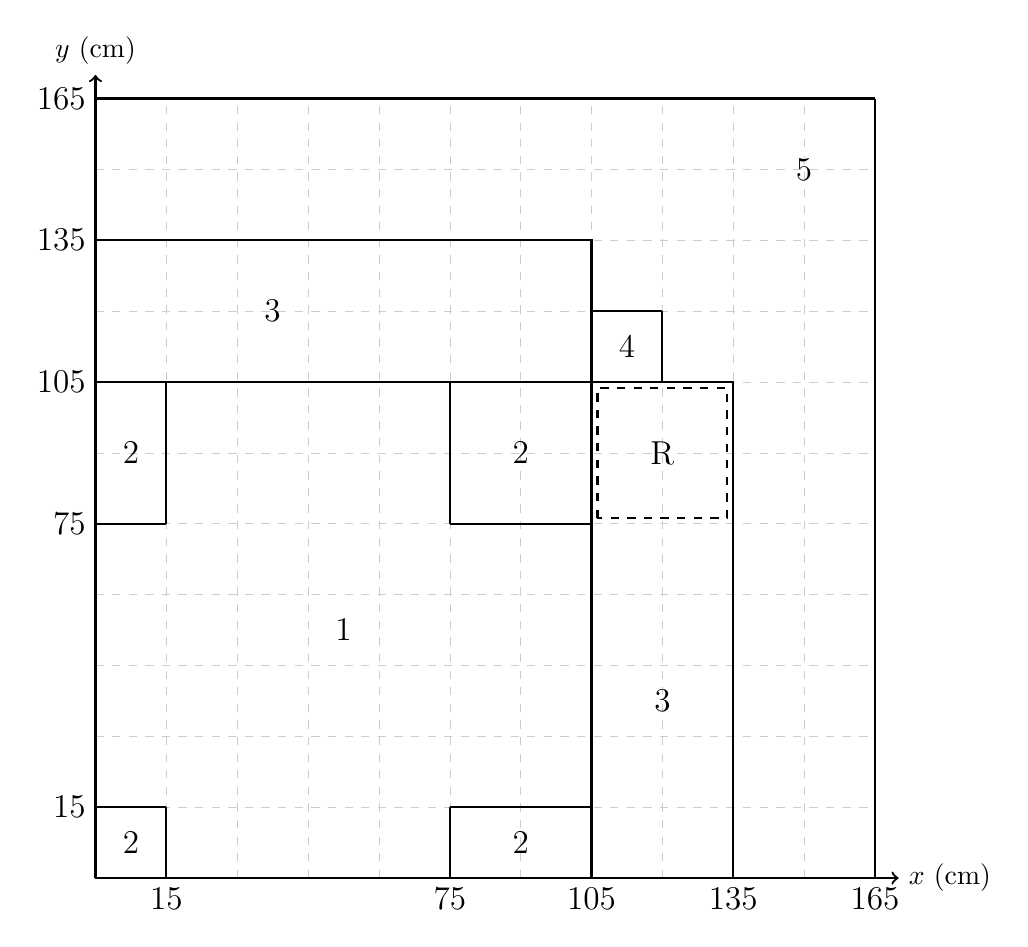
\begin{tikzpicture}[scale=0.6]
	
	\begin{scope}<->;
	
	% GRID
	\draw[step=1.5cm,gray,very thin, dashed,opacity=0.4] (0, 0) grid (16.5,16.5);
	
	% AXES
	\draw[black, thick, ->] (0, 0) -- (17,  0) node[right] {$x$ (cm)};
	\draw[black, thick, ->] (0, 0) -- ( 0, 17) node[above] {$y$ (cm)};
	
	% Material 1 regions 
	
	\node[font=\large] at (5.25, 5.25) {1};
	
	% Material 2 regions
	\draw[black, thick] (0, 1.5) -- (1.5, 1.5);
	\draw[black, thick] (1.5, 0) -- (1.5, 1.5);
	\node[font=\large] at (0.75, 0.75) {2};
	
	\draw[black, thick] ( 7.5, 0.0) -- ( 7.5, 1.5);
	\draw[black, thick] (10.5, 0.0) -- (10.5, 1.5);
	\draw[black, thick] ( 7.5, 1.5) -- (10.5, 1.5);
	\node[font=\large] at (9.0, 0.75) {2};
	
	\draw[black, thick] ( 0.0,  7.5) -- ( 1.5,  7.5);
	\draw[black, thick] ( 0.0, 10.5) -- ( 1.5, 10.5);
	\draw[black, thick] ( 1.5,  7.5) -- ( 1.5, 10.5);
	\node[font=\large] at ( 0.75, 9.0) {2};
	
	\draw[black, thick] ( 7.5,  7.5) -- ( 7.5, 10.5);
	\draw[black, thick] ( 7.5,  7.5) -- (10.5,  7.5);
	\draw[black, thick] (10.5, 10.5) -- ( 7.5, 10.5);
	\draw[black, thick] (10.5, 10.5) -- (10.5,  7.5);
	\node[font=\large] at ( 9.0, 9.0) {2};
	
	% Material 3 regions
	\draw[black, thick] (10.5,  0.0) -- (10.5, 10.5) -- (13.5, 10.5) --  (13.5,  0.0) -- (10.5,  0.0);
	\node[font=\large] at ( 12.0, 3.75) {3}; 
	\draw[black, thick] (0.0, 10.5) -- (10.5, 10.5) -- (10.5, 13.5) -- (0.0, 13.5) --  (0.0, 10.5);
	\node[font=\large] at ( 3.75, 12.0) {3}; 
	
	% Material 4 regions  
	\draw[black, thick] ( 12,  12) -- ( 12, 10.5) -- (10.5, 10.5) -- (10.5,  12) -- ( 12,  12);
	\node[font=\large] at ( 11.25,11.25) {4};
	
	
	% Material 5 regions
	\draw[black, thick] ( 16.5,  0.0) -- (16.5, 16.5);
	\draw[black, thick] (  0.0, 16.5) -- (16.5, 16.5);
	\node[font=\large] at (15.0, 15.0) {5};
	
	% Perturbed regions
	\def\eps{0.125}
	\draw[black, thick, dashed] (10.5+\eps, 7.5+\eps) -- (10.5+\eps, 10.5-\eps) -- (13.5-\eps, 10.5-\eps) -- (13.5-\eps, 7.5+\eps) --  (10.5+\eps, 7.5+\eps);
	
	\node[font=\large] at (12,9) {R};
	
	% ticks
	\foreach \x/\xtext in {15, 75, 105, 135, 165}
	\draw[black,xshift=0.1*\x cm] (0,.3) -- (0,0) node[below, font=\large] {$\xtext$};
	\foreach \y/\ytext in {15, 75, 105, 135, 165}
	\draw[black,yshift=0.1*\y cm] (.3,0) -- (0,0) node[left, font=\large] {$\ytext$};
	\end{scope}
	\end{tikzpicture}
	\caption{Schematic of LRA benchmark.}
	\label{fig:lra core}
\end{figure}
The transient is initiated by a control rod ejection with constant velocity over a period of 2 seconds leading to a super-critical, prompt transient, in which the power increases by about 10 orders of magnitude in a very short time.
The control rod movement is represented by changing the thermal absorption cross section of the control rod material.
In this application, the two-group diffusion equation represented in Sec.~\ref{sec:fom}, is coupled with thermal feedback through adiabatic fuel heat-up defined by
\begin{equation}
	\frac{\partial}{\partial t}T(x,t) = \alpha[\Sigma_{f1}(x,t)\phi_1(x,t)+\Sigma_{f2}(x,t)\phi_2(x,t)] \, ,
	\label{eq:heatup}
\end{equation}
and corresponding Doppler feedback defined by
\begin{equation}
	\Sigma_{a1}(x,t) = \Sigma_{a1}(x,t=0)[1+\gamma(\sqrt{(T(x,t)}-\sqrt{(T_0)})] \, ,
	\label{eq:doppler}
\end{equation}
where $\Sigma_{f_i}$ is the fission cross section of group $i$, $T$ is the temperature, $\Sigma_{a1}$ is the fast absorption cross section and $T_0$ is the initial temperature which is $300 $ K,
$\alpha = 3.83\times 10^{-11}~\text{K}~\text{cm}^3$ and $\gamma = 3.034\times 10^{-3} ~\text{K}^{-0.5}$.
The power local is computed as
\begin{equation}
	P(x,t)=\kappa [\Sigma_{f1}(x,t)\phi_1(x,t)+\Sigma_{f2}(x,t)\phi_2(x,t)] \, ,
\end{equation}
where $\kappa = 3.204\times 10^{-11}~ \text{W/fission}$.
The model was implemented in the deterministic transport code Detran~\cite{roberts2014advanced}.
A mesh-centered, finite-difference discretization was used in space, while a first-order, backward-difference temporal discretization was used with a fixed 0.001 s step size.  
The initial condition for the transient was computed by solving the steady-state equation, for which $k_{\text{eff}}$ was found to be 0.9975.
Note that at each time step the fast absorption cross section is a function of the solution itself.
The convergence criterion used to reduce the $\text{L}_2$ norm  of the relative flux error between two consecutive iterations to less than $1\times 10^{-6}$, or
\begin{equation}
	\|\frac{\mathbf{\Phi}^{i+1} - \mathbf{\Phi}^{i}} {\mathbf{\Phi}^i}\| \le  1\times 10^{-6} \, ,
	\label{eq:convergance criteria} 
\end{equation}
where the superscript $i$ denotes the iteration number.
The transient was calculated for 3.0 seconds.
Figure~\ref{fig:lra fom power} shows the reference full-order model power along with the core average temperature.
This reference solution is not necessarily numerically converged in either space or time but represents the simulation response that one wishes to approximate.
\begin{figure}[h!]
	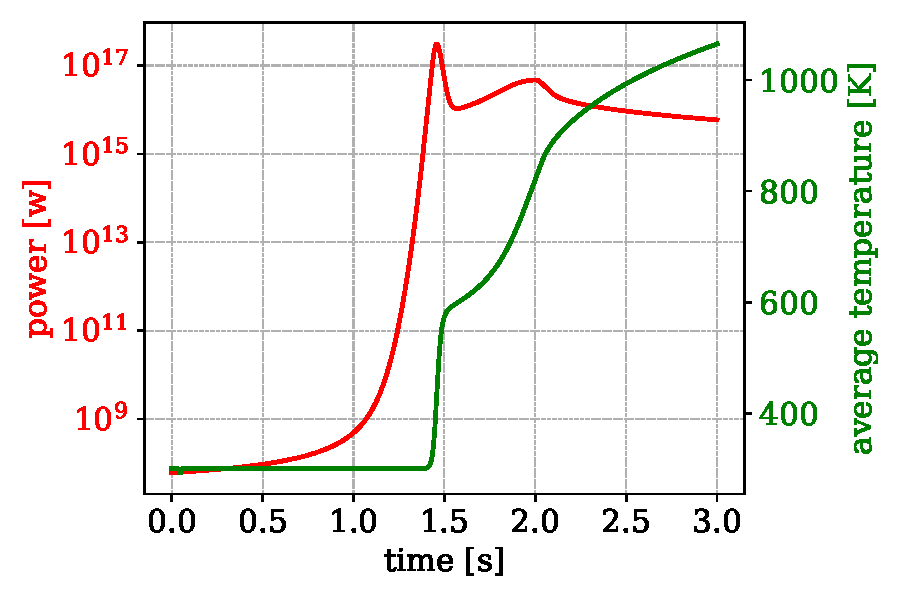
\includegraphics[width=1.0\linewidth]{../figures/LRA_fom_power_temperature.pdf}
	\caption{LRA core power}
	\label{fig:lra fom power}
\end{figure}

%\begin{figure}[H]
%	\centering
%	\begin{subfigure}[b]{0.7\textwidth}
%		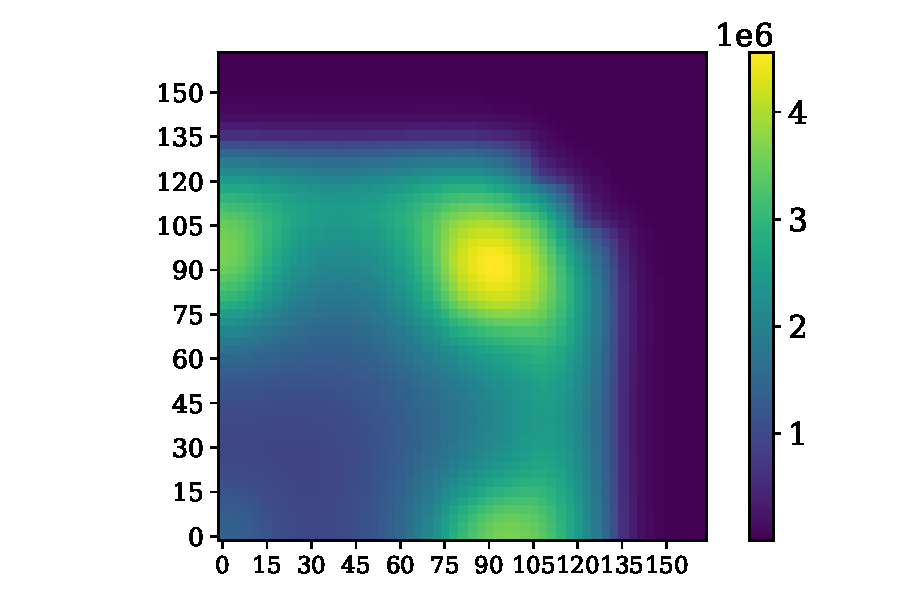
\includegraphics[width=1.0\linewidth]{../figures/ss_fom_fast_flux_image.pdf}
%		\caption{Steady state fast flux.}
%		\label{fig:ss fast flux}
%	\end{subfigure}
%	\begin{subfigure}[b]{0.7\textwidth}
%		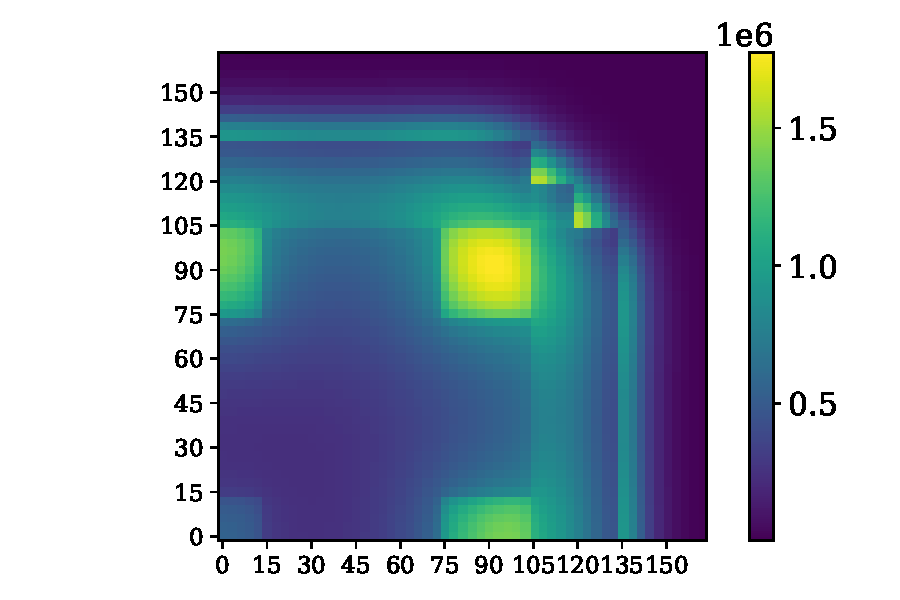
\includegraphics[width=1.0\linewidth]{../figures/ss_fom_thermal_flux_image.pdf}
%		\caption{Steady state thermal flux.}
%		\label{fig:ss thermal flux}
%	\end{subfigure}
%	\caption{Steady state group flux $(\text{neutrons} ~\text{cm}^2/s)$}
%	\label{fig:lra ss flux}
%\end{figure}

\begin{table}[H]
	\begin{threeparttable}	
		\centering
		\begin{tabular}{c|l|l|l|l|l}
			material & group  & $D$ (cm) & $\Sigma_{a} ~ (\text{cm}^{-1})$ & $\Sigma_{s2\gets 1}~ (\text{cm}^{-1})$ & $\nu\Sigma_{f}~ (\text{cm}^{-1})$ \\
			\hline
			\multirow{2}{*}{1}& 1   & 1.255  &  0.008252   & 0.004602 &  \multirow{2}{*}{0.02533} 	\\
			& 2   & 0.211  &  0.1003     &  0.1091  &  \\
			\hline
			\multirow{2}{*}{2}& 1   & 1.268  &  0.007181    & 0.004609  & \multirow{2}{*}{0.02767}  \\	
			& 2   & 0.1902 &  0.07047     & 0.08675   &  \\
			\hline
			
			\multirow{2}{*}{3}& 1   & 1.259  &  0.008002    & 0.004663 & \multirow{2}{*}{0.02617} \\	
			& 2   & 0.2091 &  0.08344     &   0.1021 &                          \\
			\hline
			\multirow{2}{*}{4}& 1   & 1.259  &  0.008002    & 0.004663 &  \multirow{2}{*}{0.02617} \\	
			& 2   & 0.2091 &  0.073324    & 0.1021   &                           \\
			\hline
			\multirow{2}{*}{5}& 1   & 1.257  &  0.0006034   &   0.0    & \multirow{2}{*}{0.04754}\\	
			& 2   & 0.1592 &   0.01911    &   0.0    &  \\
			\hline
		\end{tabular}
		\begin{tablenotes}
			\item $v_1 = 3\times10^{7} ~\text{cm/s} $,  $v_2 = ~3\times10^{5} \text{cm/s}.$.
		\end{tablenotes}
	\end{threeparttable}
	\caption{Two group constants of the LRA benchmark.}
\end{table}


\begin{table}[H]
	\centering
	\begin{tabular}{c|l|l}
		group & $\beta_i$  & $\lambda_i$ ($s^{-1}$)  \\
		\hline
		1    &  0.0054 & 0.00654 \\
		2    &  0.001087 & 1.35  \\
		\hline
	\end{tabular}
	\caption{Delayed neutron data of the LRA benchmark.}
	\label{tab:precursor data}
\end{table}

%--------------------------------------------------------------------------------------------------------------%

\section{ROM }
\subsection{ROM Implementation}

The POD-Galerkin projection procedures described in Sec.~\ref{sec:POD} were applied to the system in Eq.~\ref{eq:transient fom} to approximate the group flux and the core power of the LRA benchmark with increasing the spatial fidelity, i.e, spatial grids of $22\times 22$, $44\times44$ and $55 \times 55$ were used.\\
POD basis set was generated for each group flux while one basis set was generated for both precursors groups, i.e, 
$\mathbf{\Phi}_1(t) = \mathbf{U}_1\mathbf{a}_1(t)$, $\mathbf{\Phi}(t)_2 = \mathbf{U}_2\mathbf{a}_2(t)$ and $\mathbf{C}(t) = \mathbf{U}_c\mathbf{a}_c(t)$, where the $\mathbf{U}_1$, $\mathbf{U}_2$  and $\mathbf{U}_c$ are the POD bases of the fast group, thermal group and precursor concentration respectively, and $\mathbf{a}_1$, $\mathbf{a}_2$ and $\mathbf{a}_c$ are their respective temporal coefficients. 
The resulting ROM can be represented as 
\begin{equation}
	\frac{d\mathbf{\hat{y}}}{dt} = \mathbf{A}_r\mathbf{\hat{y}}\, , 
	\label{eq:ROM}
\end{equation}
where
 \begin{equation*}
	\mathbf{\hat{y}} = \begin{pmatrix}
	\mathbf{a}_1\\
	\mathbf{a}_2 \\
	\mathbf{a}_c \\
	\end{pmatrix} \,.
 \end{equation*}
%The first 100 normalized singular values \footnote{The normalization is done be dividing each singular value by the sum of all singular values.} of the group flux are shown in Fig.~\ref{fig:lra singular values}.

For POD rank selection, the ROM was solved with different flux ranks and the mean relative L$_2$ flux errors are computed and are shown in Fig.~\ref{fig:POD flux rank}.
\begin{figure}[h!]
	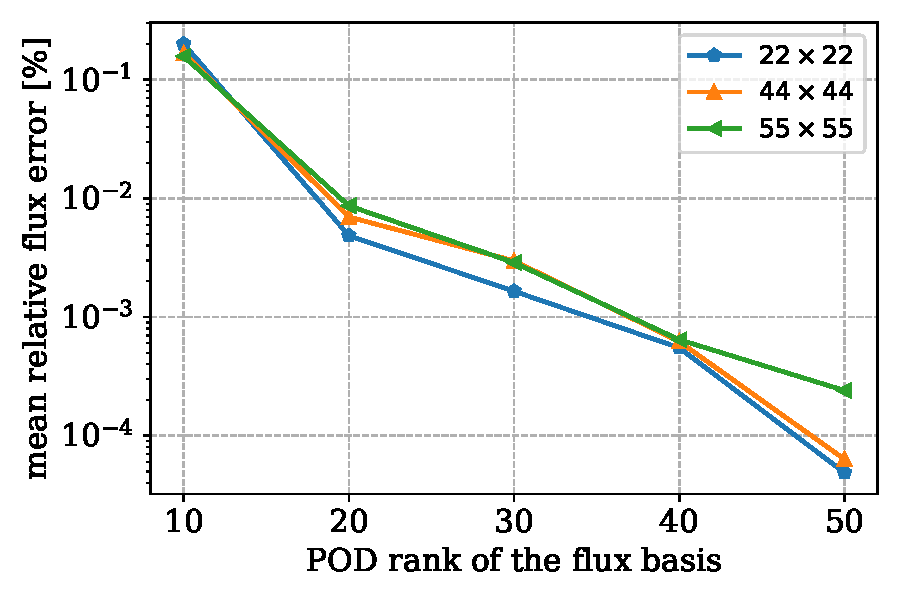
\includegraphics[width=1.0\linewidth]{../figures/flux_rank_convergence.pdf}
	\caption{flux normalized singular value.}
	\label{fig:POD flux rank}
\end{figure}
A POD rank of 30 was selected fore each group flux since it results in a reasonably good error, i.e, less than 0.001\% and the same rank was used for approximating the precursors concentration.
Higher ranks can be selected if a better ROM accuracy is desired.
Furthermore, a ROM was constructed for the coupled thermal feedback model and the temperature field was approximated by projecting it onto a lower dimensional POD space
\begin{equation}
	\mathbf{T}(t) = \mathbf{U}_{\text{temp}}\mathbf{a}_T(t) \, ,
	\label{eq:temp pod}
\end{equation}
where $\mathbf{U}_{\text{temp}}\in\mathbb{R}^{n \times r_T} $ is the POD subspace of rank $r_T$ and $\mathbf{a}_T\in \mathbb{R}^{r_T}$ is a vector of the corresponding temporal coefficients. 
%To obtain the subspace, snapshots of the temperature were collected at different times for which the SVD was computed.
%Shown in Fig.~\ref{fig:lra T singular values} are the first 100 normalized singular values.
Inserting Eq.~\ref{eq:temp pod} into Eq.~\ref{eq:heatup} and multiplying on the left by $\mathbf{U}_T^T$ \footnote{The superscript T denotes the matrix transpose.} yields
\begin{equation}
	\frac{d\mathbf{a}_T(t)}{dt}  = \alpha [\underbrace{\mathbf{U}_{\text{temp}}^T \boldsymbol{\Sigma}_{f1}\mathbf{U}_1}_{\mathbf{U}_{T1}}\mathbf{a_1}(t) + \underbrace{\mathbf{U}_{\text{temp}}^T\boldsymbol{\Sigma}_{f2}\mathbf{U}_2}_{\mathbf{U}_{T2}}\mathbf{a_2}(t)] \, .
	\label{eq:reduced temp}
\end{equation}
Note that $\mathbf{U}_{T1}$ and $\mathbf{U}_{T2}$ are time-independent, so they can be precomputed once and stored.
For selecting the temperature rank, i.e, $r_T$, the ROM was solved with different temperature ranks and the selected flux and precursors ranks.
The mean core power relative error was computed in each case and is shown in Fig.~\ref{fig:temperature rank} based on which a POD of rank $10$ was selected for approximating the temperature since there was no improvement in the error for the higher ranks.

\begin{figure}[H]
	\centering
	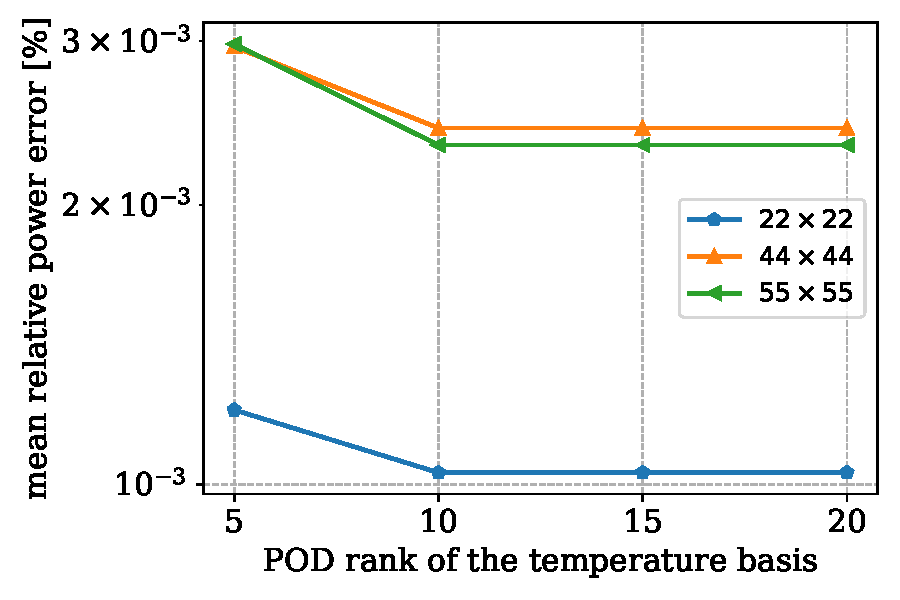
\includegraphics[width=1.0\linewidth]{../figures/temperature_rank_convergence.pdf}
	\caption{temperature normalized singular value.}
	\label{fig:temperature rank}
\end{figure}

Now to solve for the quantities of interest, the flux temporal coefficients (i.e, $\mathbf{a_1}(t)$ and $\mathbf{a_2}(t)$) are computed at each time step by solving the reduced system in Eq.~\ref{eq:ROM} and then used to compute the temperature coefficients by employing a first-order, backward-difference scheme to Eq.~\ref{eq:reduced temp}.
Similar to the full-order model, a fixed point iteration is used to treat the flux non-linearity.
However, it was observed that the reduced model needed more iterations to converge which could be due to the small value of some of the flux coefficients, hence a convergence criteria was employed based on the relative $\text{L}_2$ norm of the error of flux coefficients between two consecutive iterations 
\begin{equation}
	\frac{\|\mathbf{a}^{i-1} - \mathbf{a}^{i}\|}{\|\mathbf{a}_i \|} \le 1\times 10^{-6}  \, , 
\end{equation}

%Note that the fast absorption cross section needs to be updated at each time step using Eq.~\ref{eq:doppler} in which the core temperature distribution is required.
%In order to avoid reconstructing the full order temperature, 
%the DEIM was used to approximate the absorption cross section.
%For this purpose, snapshots of which were collected in order to generate a POD subspace that is used to approximate its space and to find a set of interpolation indices as illustrated in Algorithm~\ref{alg:DEIM}.
%DEIM of order $10$ was used and hence, the cross section was reconstructed at each time step at only 10 points in the spatial space.
Since the reactivity insertion was simulated by changing the absorption cross section, the operator $\mathbf{A}$ in Eq.~\ref{eq:transient fom} exhibits time dependence.
In particular, the submatrix $\mathbf{L}$ of $\mathbf{A}$ is the one that changes with time.
Thus, to avoid performing the expensive projection at each time step, 
The MDEIM was used to decompose the matrix $\mathbf{L}$.
Shown in Fig.~\ref{fig:lra L singular values} are the singular values resulting from the SVD of the serialized operator snapshots. 
A MDEIM of order $15$ was used since the singular-values decay by large magnitude around this value, however, higher orders can be chosen for higher accuracy.

\begin{figure}[H]
	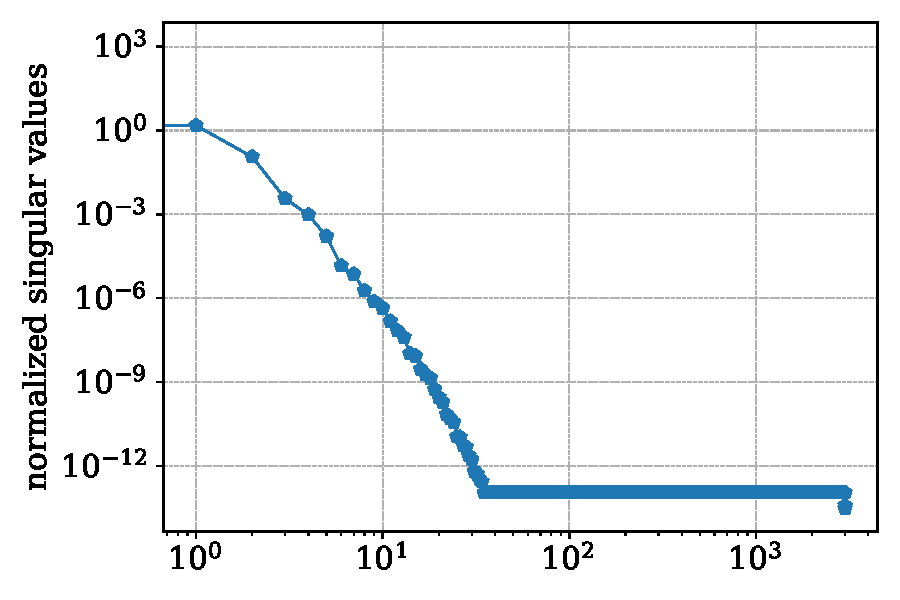
\includegraphics[width=1.0\linewidth]{../figures/LRA_L_singular_values.pdf}
	\caption{The normalized singular values of the serializes operator $\mathbf{L}$.}
	\label{fig:lra L singular values}
\end{figure}
%----------------------------------------------------------------------------------------------------%

\subsection{ROM results}

Using the selected ranks in the previous subsection, MDEIM-ROMs were developed for full-order models of spatial grids $22\times 22$, $44\times44$ and $55 \times 55$.
%For brevity, we show the first four POD modes with their temporal coefficients of only the $55 \times 55$ grid in Fig.~\ref{fig:lra flux modes}.
%\begin{figure}[H]
%	\centering
%	\begin{subfigure}[b]{0.45\textwidth}
%		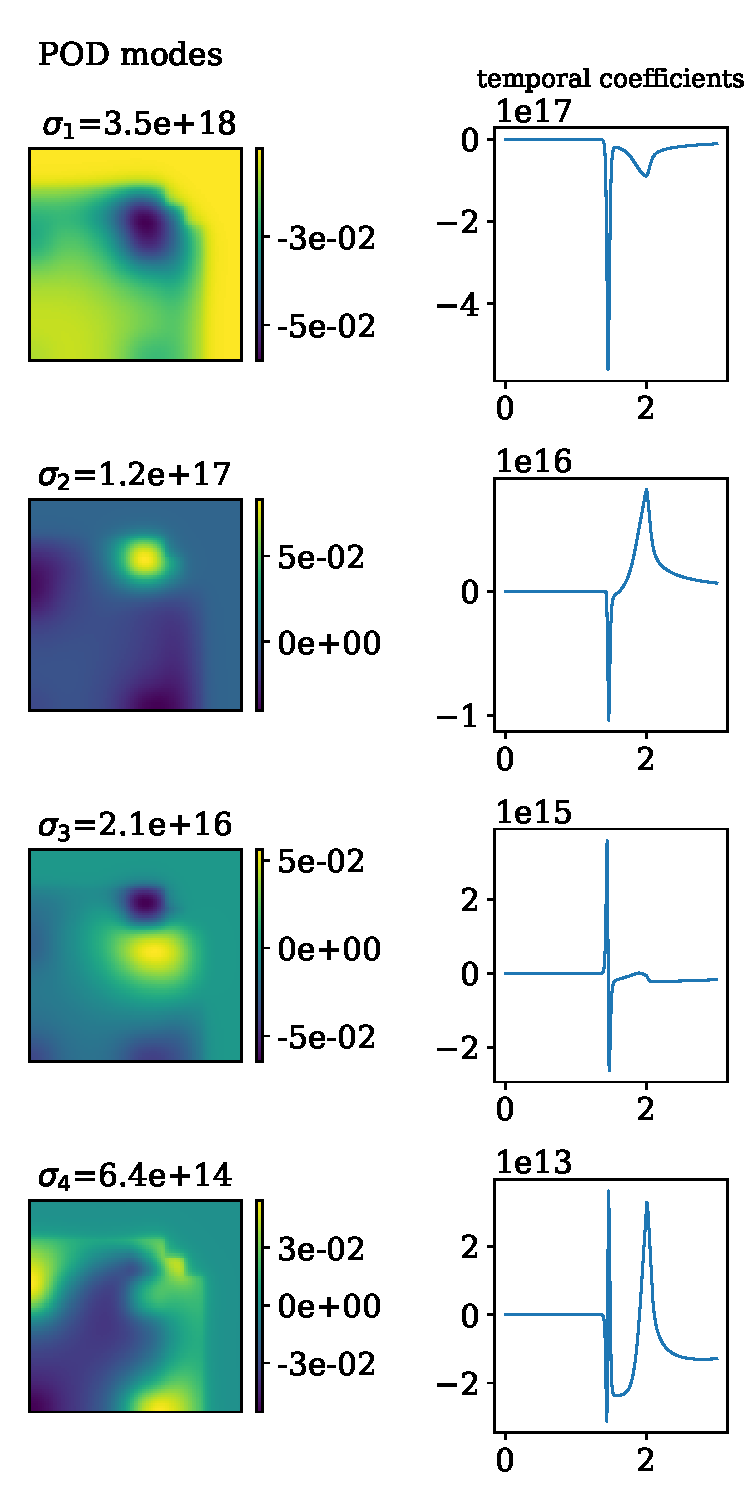
\includegraphics[width=1.0\linewidth]{../figures/LRA_fast_modes.pdf}
%		\caption{Fast flux modes.}
%		\label{fig:ss fast flux 2}
%	\end{subfigure}
%	\begin{subfigure}[b]{0.45\textwidth}
%		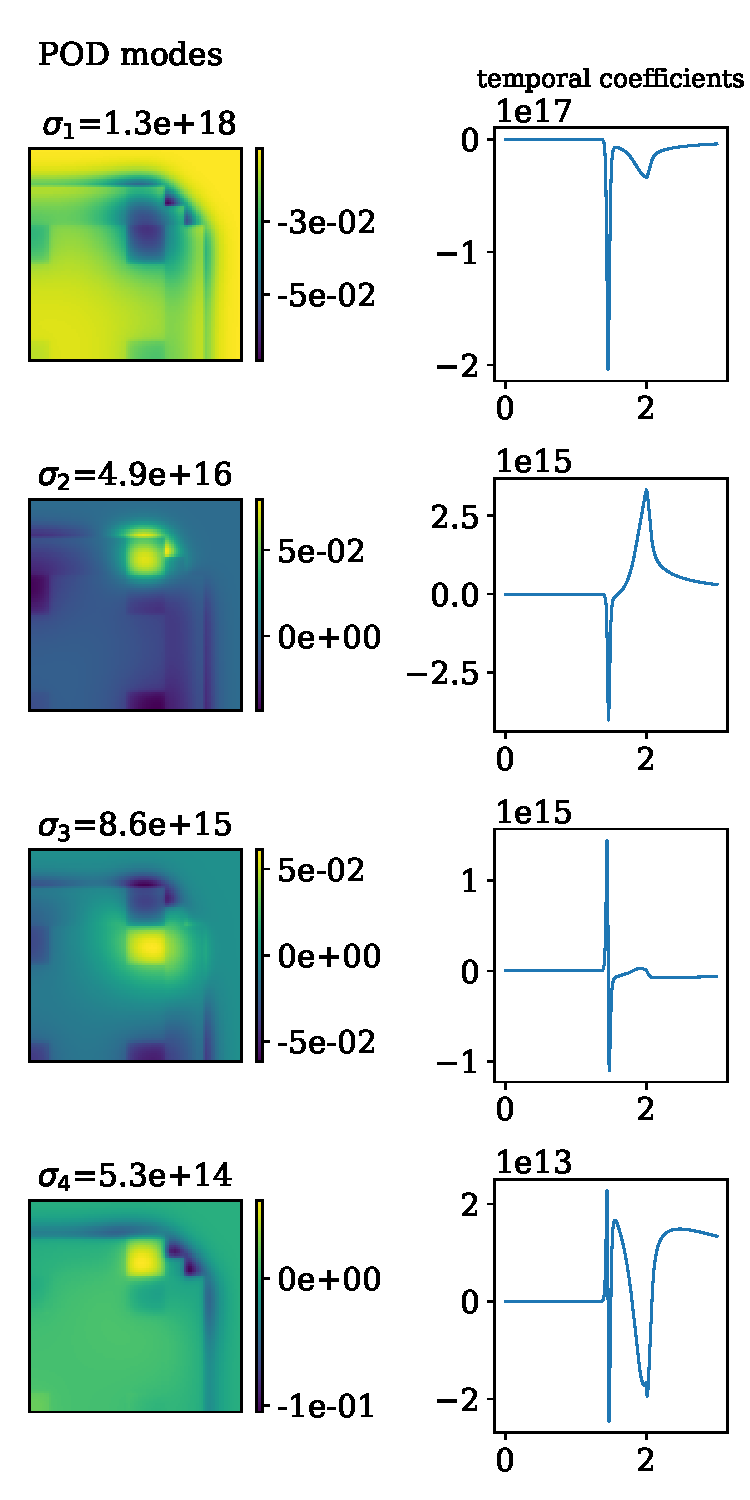
\includegraphics[width=1.0\linewidth]{../figures/LRA_thermal_modes.pdf}
%		\caption{Thermal flux modes.}
%		\label{fig:ss thermal flux 2}
%	\end{subfigure}
%	\caption{Flux POD modes and their temporal coefficient.}
%	\label{fig:lra flux modes}
%\end{figure}
The ROMs were solved for the group flux from which the core power was computed.
The absolute relative error in the predicted core powers are shown in Fig.~\ref{fig:deim power error}.

\begin{figure}[H]
	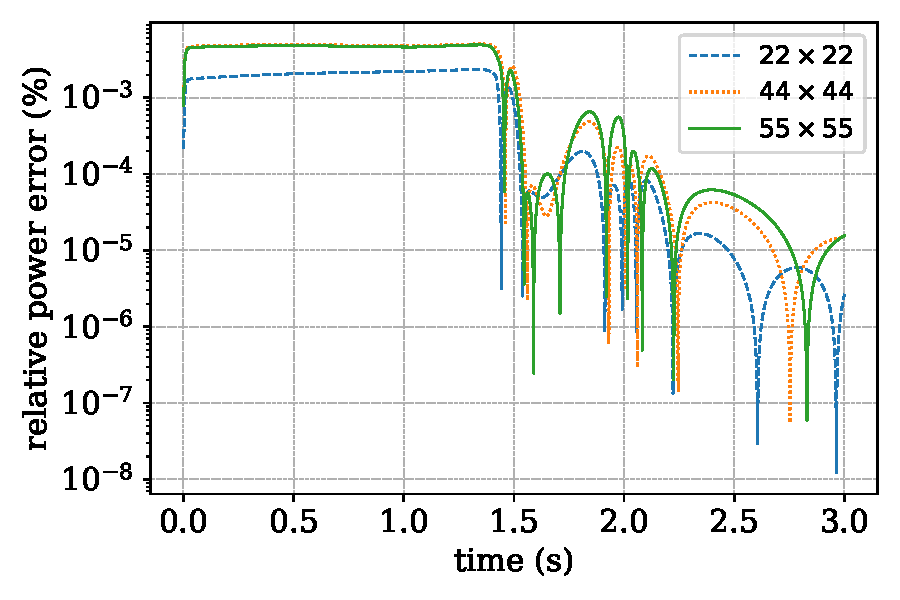
\includegraphics[width=1.0\linewidth]{../figures/LRA_power_deim_relative_error.pdf}
	\caption{Relative error of the power predicted by MDEIM-ROM}
	\label{fig:deim power error}
\end{figure}

To understand the impact of employing the MDEIM on the error; the results are compared with these of a direct projection ROM, i.e., with performing direct operator projection at each time step.
The relative difference of the power between both models is shown in Fig.~\ref{fig:rom-deim power error}.
The shown errors implies that MDEIM accurately approximates the problem operator.

\begin{figure}[H]
	\centering
	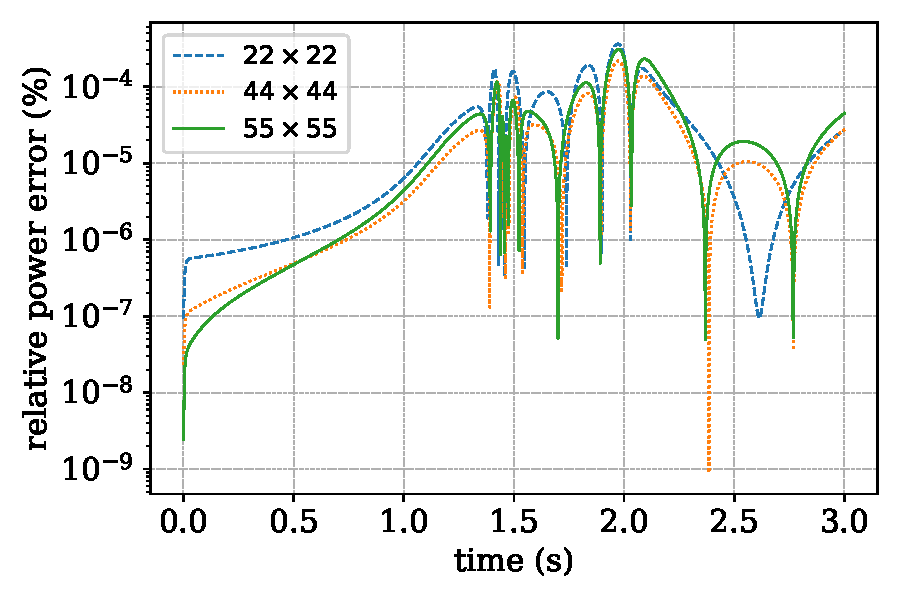
\includegraphics[width=1.0\linewidth]{../figures/LRA_mdeim_relative_error.pdf}
	\caption{Relative difference in the predicted power between the direct projection ROM and the MDEIM-ROM.}
	\label{fig:rom-deim power error}
\end{figure}
Also, the spatial-averaged relative error in the approximated temperature was computed and is shown in Fig.~\ref{fig:deim tempearture error}.

\begin{figure}[H]
	\centering
	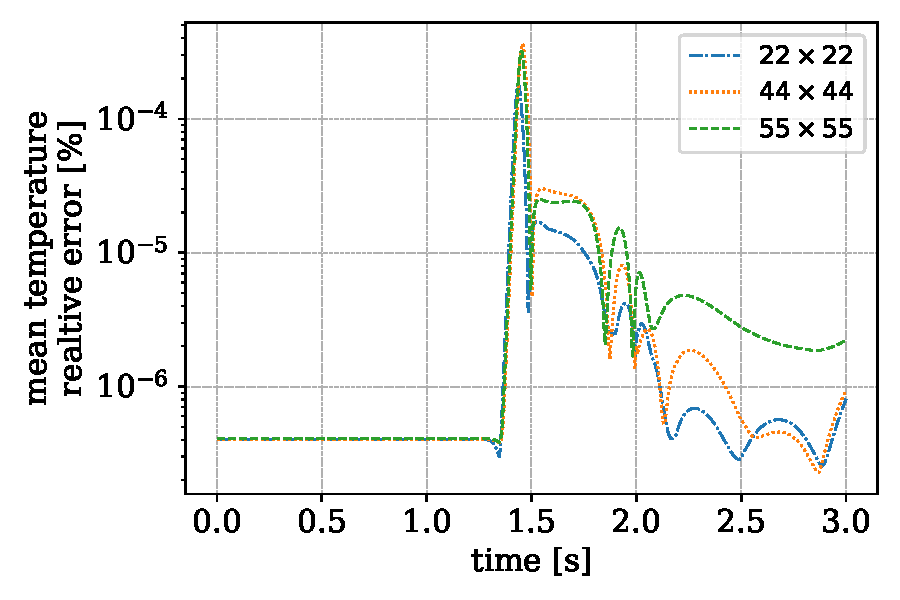
\includegraphics[width=1.0\linewidth]{../figures/temperature_relative_error.pdf}
	\caption{Relative error of the temperature predicted by ROM.}
	\label{fig:deim tempearture error}
\end{figure}
%As mentioned earlier, the non-linearity of the fast absorption cross section was approximated using DEIM of rank 10.
%Shown in Fig.~\ref{fig:cross section deim indices} are the ten selected interpolation points onto the absorption cross section map at the end of transient, i.e., at $t=3$ s.
%The temperature was constructed only at these locations from which the cross section is evaluated using Eq.~\ref{eq:doppler}.
%\begin{figure}[H]
%	\centering
%	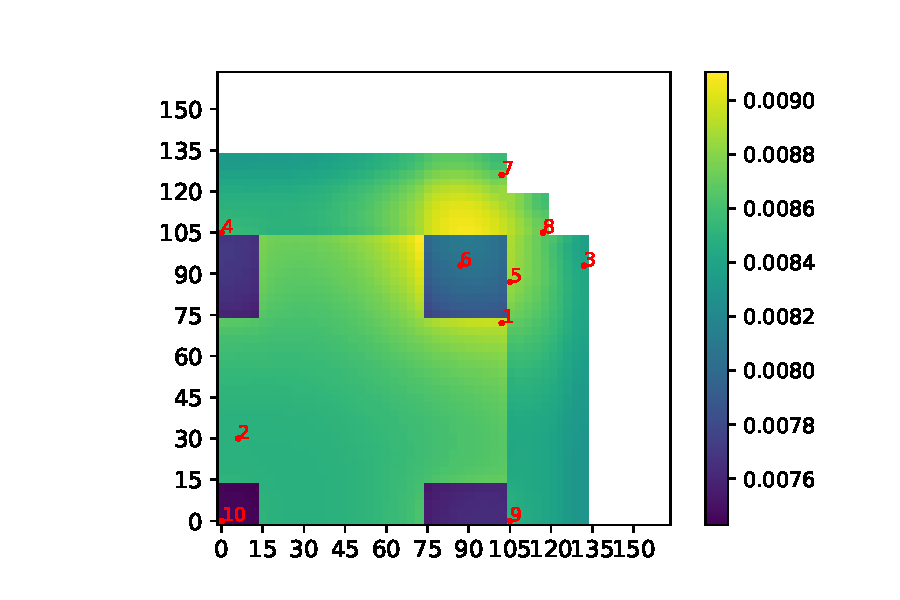
\includegraphics[scale=1.2]{../figures/LRA_XS_interpolation_points_XS_map.pdf}
%	\caption{The fast cross section at t=3 s with the selected interpolation indices in red color.}
%	\label{fig:cross section deim indices}
%\end{figure} 
To further assess the performance of the ROM, the relative error in a local quantity such as the assembly power at the peak is computed and is shown in Fig.~\ref{fig:assembly power error fm=5} for the $55\times 55$ grid from which it can be seen that the maximum error is in the order of $1\times 10^{-5}\%$.

\begin{figure}[H]
	\centering
	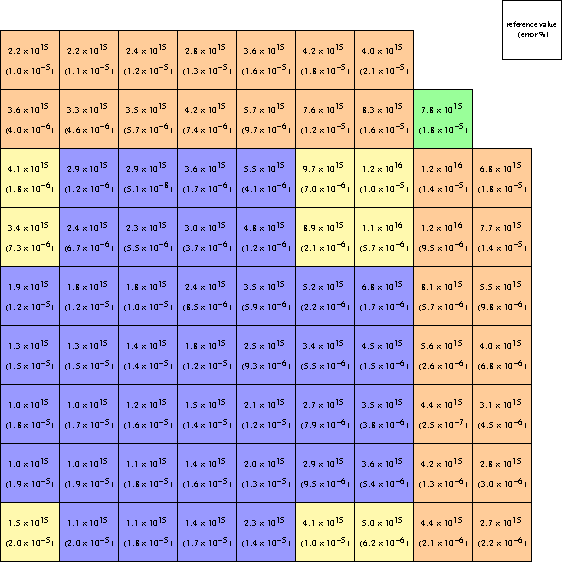
\includegraphics[width=0.7\linewidth]{../figures/lra_assemb_fm=5.pdf} 
	\caption{Assembly-averaged power relative error for the $55\times 55$ grid}
	\label{fig:assembly power error fm=5}
\end{figure} 

Moreover, the computational times of the FOM and the ROMs are given in Table~\ref{table:cpu time}.

\begin{table*}[h!]
	\centering
	\caption{Computational time of the FOM and the ROMs for the LRA benchmark.}
	\label{table:cpu time}
	\begin{tabular}{c|c|c|c}  
		Grid &	FOM (s)   &  direct projection ROM (s) & MDEIM-ROM (s)    \\
		\hline
		$22\times 22$ &  243   & 76   & 38   \\
		$44\times 44$ &  1269  & 226   & 46   \\
		$55\times 55$ &  2195  & 341   & 50   \\
		\hline
	\end{tabular}
\end{table*}

Notably, the MDEIM-ROM is cheaper than the direct projection ROM with a speed-up that depends on the original model size.
More importantly, the MDEIM-ROM cost is slightly dependent on the problem dimension while the other ROM time increases with the grid size because the operator projection is performed at each time step.
The shown MEDIM-ROM time includes the offline cost which involves the operator $\mathbf{L}$ decomposition and the projection of the decomposed matrices.
Also, both the ROMs times include the time to reconstruct of the full-order solution.

%------------------------------------------------------------------------------------------------%
\subsubsection{Parametric ROM Results}

In the previous section, the developed ROM was used to reconstruct the solution using a POD subspace obtained from snapshots generated using the same parameter point at which the solution is sought.
Here, our purpose is to extend the capability of the developed ROM to perform parametric studies.
However, it is important to clarify that it is not our goal in this study to quantify output uncertainties or perform statistical analysis.
Instead, we merely aim to measure the prediction error of the ROM at new parameter points using a POD subspace sampled from a parameter domain of interest.
A case study was performed in which the parameters of interest are assumed to be the kinetic data, i.e., the delayed neutron fractions and the decay constants. A POD greedy sampling was used to construct a global POD subspace.
Although the original benchmark employs two precursor groups, it was more convenient in this study to use six groups to enlarge the parameter space.
Shown in Table \ref{tab: 6 groups precursor data} are the parameters normal distributions data adopted from Refs.~\cite{keepin1957delayed, tuttle1975delayed}.
A POD greedy sampling is used for which a set of 50 parameters points were generated to obtain a global POD space, where at each iteration, three POD basis vectors are added to the space.
A grid of $22\times 22$ is used throughout this study.
A greedy algorithm stopping criteria was used such that the iteration terminates if the relative norm of the flux error is $1\times10^{-4}$ or the POD space has a size of 6 (i.e., 20 parameters points are selected).
As noted earlier, there are no general prior criteria for selecting these parameters.

\begin{table}[h!]
	\centering
	\begin{tabular}{c|l|l}
		group i& $\beta_i \pm \sigma_{\beta_i}$  & $\lambda_i\pm \sigma_{\lambda_i} (s)^{-1}$)  \\
		\hline
		1    &  $0.038\pm 0.004$ & $0.0127 \pm 0.0003$ \\
		2    &  $0.213 \pm 0.007$  & $0.0317 \pm 0.0012$ \\
		3    &  $0.188 \pm 0.024$ & $0.1150 \pm 0.0040$ \\
		4    &  $0.407 \pm 0.010$ & $0.3110 \pm 0.0120$ \\
		5    &  $0.128 \pm 0.012$ & $1.4000\pm0.1200$ \\
		6    &  $0.026\pm0.004$ & $3.8700\pm0.5500$ \\
	\end{tabular}
	\caption{6 groups delayed neutron precursor data.}
	\label{tab: 6 groups precursor data}
\end{table}

The MDEIM-ROM is sought to predict the power at every $0.001$ s during the transient, however, a time step of $0.005$ s was used in the greedy procedures.
Shown in Fig.~\ref{fig:lra greedy error} is the flux error convergence with the greedy iterations.
As shown, the maximum size of the POD space, i.e., 60, is reached before the error approaches the specified tolerance.
The resulting POD basis was stored and used for testing the ROM.

\begin{figure}[H]
	\centering
	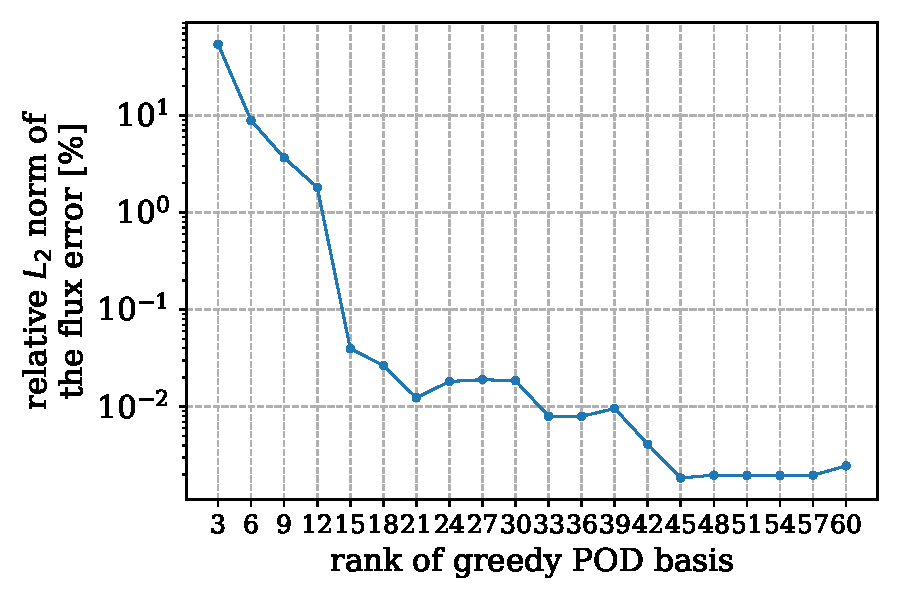
\includegraphics[width=0.9\linewidth]{../figures/greedy_convergance.pdf}
	\caption{Greedy error convergance}
	\label{fig:lra greedy error}
\end{figure}

Thus, 50 new parameter samples were generated, and the ROM was executed with the resultant greedy basis.
Moreover, the FOM was run at these testing parameter points, and the error between both models was computed.
The quantities of interest were the assembly power at the peak and the maximum core temperature, i.e., the end-of-transient temperature.
Note that the time to peak is different from sample to sample.
Shown in Fig.~ \ref{fig:peak power mean error}, the sample mean of the assembly power error, at the peak, where the mean core maximum temperature error is shown in Fig.~\ref{fig:T mean error}.

\begin{figure}[H]
	\centering
	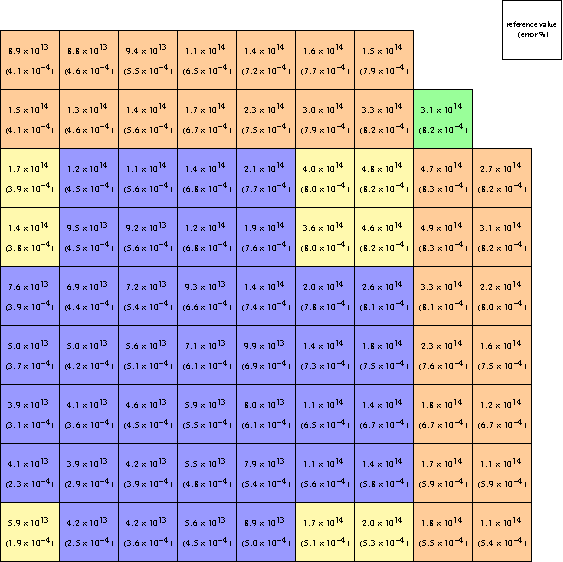
\includegraphics[scale=1]{../figures/LRA_power_mean_err.pdf}
	\caption{Sample mean of the core peak power}
	\label{fig:peak power mean error}
\end{figure}

\begin{figure}[H]
	\centering
	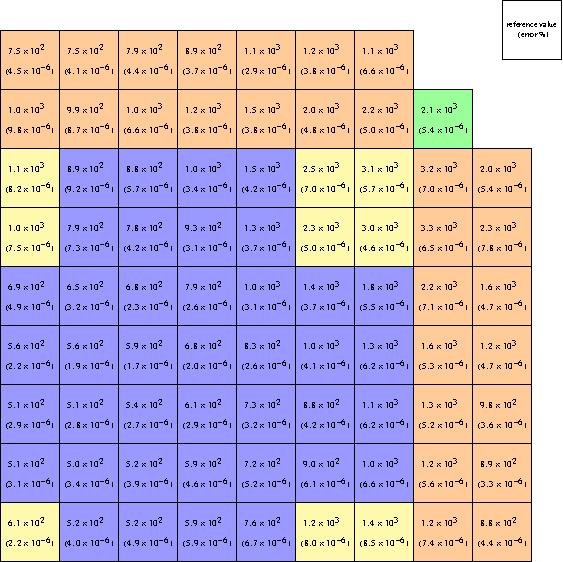
\includegraphics[scale=1]{../figures/LRA_T_mean_err_peak.pdf}
	\caption{Sample mean of the core maximum temperature}
	\label{fig:T mean error}
\end{figure}
Among all samples, the maximum assembly power peak was $0.00111\%$, and the maximum temperature error was $2.9\times10^{-5}\%$.
The resulting errors imply that the greedy-sampled POD subspace is rich with information from the whole parameters domain,
and accordingly, resulted in a good approximation even for parameters not among the training sample.

%------------------------------------------------------------------------------------------------------%
\section{Conclusion}

In this work, we developed a ROM to approximate neutronic transients with a lower computational cost.
The main focus was treating non-linear models since they pose a challenge in terms of the computational cost even with using reduced-order models.
The computational complexity associated with the ROM arises from requiring the problem operator to be projected at each iteration within the time step.
In particular, performing the projection entails a number of FLOPs that depend on the original system dimension.
Consequently, for high dimensional problems, the projection step could add significant cost to the ROM, reducing its efficiency.
The ROM was built using the POD-Galerkin projection method to reduce the number of equations to be solved, and combined with the matrix version of DEIM to alleviate the burden associated with projecting the problem operator.
The LRA benchmark representing a simplified multi-physics problem was the application used to illustrate the method.
Using the MDEIM introduced FOMs speeds up that range from 4 to 50 depending on the numerical fidelity, with a maximum power relative error in the order of $1\times 10^{-5}$\%.
More importantly, the computational saving gained from using the MDEIM-ROM is more than that of the direct projection ROM.

In general, the use of ROMs becomes more appreciable with multi-run applications that need running the model with varying input parameters.
Hence, the developed ROM was parameterized by means of POD-greedy sampling to generate a POD subspace global to a parameter domain of interest.
The parameterized ROM in which the parameters of interest were the kinetic data, resulted in a maximum assembly power relative error across all testing parameter points that is in the order of $1\times 10^{-3}$\%.

In terms of the practical implementation, an important concluding remark is that although the POD-Galerkin method is considered as an intrusive ROM technique, the implemented ROM did not require any major changes to the existing code, i.e, Detran,  making it a {\it trivially intrusive} technique.
Rather, access only to the system operator, which represents all of the underlying system discretizations, was needed.
This means that the presented ROM can be implemented in the many modern diffusion codes without making invasive changes to the working code.
%------------------------------------------------------------------------------------------------------%


\bibliography{interactnlmsample}

%%----------------------------------------------
\end{document}
